%%%%%%%%%%%%%%%%%%%%%%%%%%%%%%%%%%%%%%%%%
% Beamer Presentation
% LaTeX Template
% Version 1.0 (10/11/12)
%
% This template has been downloaded from:
% http://www.LaTeXTemplates.com
%
% License:
% CC BY-NC-SA 3.0 (http://creativecommons.org/licenses/by-nc-sa/3.0/)
%
%%%%%%%%%%%%%%%%%%%%%%%%%%%%%%%%%%%%%%%%%

%------------------------------------------------------------------------------------------------
% PACKAGES AND THEMES
%------------------------------------------------------------------------------------------------

\documentclass[table, xcolor = {dvipsnames}, 9pt]{beamer}
\usepackage{tikz}
\usetikzlibrary{calc}
\usetikzlibrary{positioning}
\usetikzlibrary{arrows.meta}
\usetikzlibrary{external}
\mode<presentation> {

% The Beamer class comes with a number of default slide themes
% which change the colors and layouts of slides. Below this is a list
% of all the themes, uncomment each in turn to see what they look like.

\usetheme{default}
%\usetheme{AnnArbor}
%\usetheme{Antibes}
%\usetheme{Bergen}
%\usetheme{Berkeley}
%\usetheme{Berlin}
%\usetheme{Boadilla}
%\usetheme{CambridgeUS}
%\usetheme{Copenhagen}
%\usetheme{Darmstadt}
%\usetheme{Dresden}
%\usetheme{Frankfurt}
%\usetheme{Goettingen}
%\usetheme{Hannover}
%\usetheme{Ilmenau}
%\usetheme{JuanLesPins}
%\usetheme{Luebeck}
%\usetheme{Madrid}
\usetheme{metropolis}
%\usetheme{Malmoe}
%\usetheme{Marburg}
%\usetheme{Montpellier}
%\usetheme{PaloAlto}
%\usetheme{Pittsburgh}
%\usetheme{Rochester}
%\usetheme{Singapore}
%\usetheme{Szeged}
%\usetheme{Warsaw}

% As well as themes, the Beamer class has a number of color themes
% for any slide theme. Uncomment each of these in turn to see how it
% changes the colors of your current slide theme.

%\usecolortheme{albatross}
%\usecolortheme{beaver}
%\usecolortheme{beetle}
%\usecolortheme{crane}
%\usecolortheme{dolphin}
%\usecolortheme{dove}
%\usecolortheme{fly}
%\usecolortheme{lily}
%\usecolortheme{orchid}
%\usecolortheme{rose}
\usecolortheme{seagull}
%\usecolortheme{seahorse}
%\usecolortheme{whale}
%\usecolortheme{wolverine}
\usefonttheme{professionalfonts}
%\setbeamertemplate{footline} % To remove the footer line in all slides uncomment this line
%\setbeamertemplate{footline}[page number] % To replace the footer line in all slides with a simple slide count uncomment this line

%\setbeamertemplate{navigation symbols}{} % To remove the navigation symbols from the bottom of all slides uncomment this line
}

\usepackage{graphicx} % Allows including images
\usepackage{booktabs} % Allows the use of \toprule, \midrule and \bottomrule in tables
\usepackage{tikz}
\usepackage{multirow}
\usepackage{natbib}
\usepackage{hyperref}
\usepackage{diagbox}
\usepackage{makecell}
\usepackage{xparse}
\usepackage{subfig}
\usepackage{amsmath}
\usepackage{amsfonts,amsthm,amsmath,amssymb}    
\usepackage{bbm}
\usepackage{bm}
\usepackage{empheq}
\usepackage{pgfplots}
\usepackage{animate}
\usepgfplotslibrary{colorbrewer}

\newcommand\mybox[2][]{\tikz[overlay]\node[fill=lightgray,inner sep=2pt, anchor=text, rectangle, rounded corners=1mm,#1] {#2};\phantom{#2}}
\hypersetup{unicode=true,
            bookmarksnumbered=true,
            bookmarksopen=true,
            bookmarksopenlevel=2,
            breaklinks=false,
            pdfborder={0 0 1},
            hypertexnames=false,
            pdfstartview={XYZ null null 1}}
\usepackage{xcolor}
\newcommand\myheading[1]{%
  \par\bigskip
  {\Large\bfseries#1}\par\smallskip}
\newcommand\given[1][]{\:#1\vert\:}
\theoremstyle{plain}
\newtheorem{thm}{Theorem}
\newtheorem{prop}{Proposition\thisthmnumber}
\newtheorem{lem}{Lemma\thisthmnumber}
\newtheorem{cor}{Corollary}
\newtheorem{defin}{Definition}
\newtheorem{algo}{Algorithm}
\newcommand*\diff{\mathop{}\!\mathrm{d}}
\newcommand*\Diff[1]{\mathop{}\!\mathrm{d^#1}}
\newcommand{\bh}[1]{{\color{blue}{#1}}}
\newcommand{\mh}[1]{{\color{magenta}{#1}}}
\newcommand{\thisthmnumber}{}
\newcommand{\tikzmark}[1]{\tikz[baseline,remember picture] \coordinate (#1) {};}
\newcommand*{\QEDA}{\hfill\ensuremath{\blacksquare}}%
\newcommand*{\QEDB}{\hfill\ensuremath{\square}}%
\DeclareMathOperator{\E}{\rm{E}}
\DeclareMathOperator{\R}{\mathbb{R}}
\DeclareMathOperator{\N}{\mathbb{N}}
\DeclareMathOperator{\Var}{\rm{Var}}
\DeclareMathOperator{\Cov}{\rm{Cov}}
\DeclareMathOperator{\Supp}{\rm{Supp}}
\DeclareMathOperator{\e}{\rm{e}}
\DeclareMathOperator{\F}{\mathcal{F}}
\DeclareMathOperator{\Z}{\mathcal{Z}}
\DeclareMathOperator{\logit}{\rm{logit}}
\DeclareMathOperator{\indep}{{\perp\!\!\!\perp}}
\DeclareMathOperator{\rank}{rank}
\DeclareMathOperator*{\argmin}{arg\,min}
\DeclareMathOperator*{\argmax}{arg\,max}
%\DeclareMathOperator{\Pr}{\rm{Pr}}
%------------------------------------------------------------------------
% TITLE PAGE
%-----------------------------------------------------------------------
\pagestyle{empty}
\title[]{Sharp null hypothesis testing} % The short title appears at the bottom of every slide, the full title is only on the title page

\author{Thomas Leavitt} % Your name
\institute[] % Your institution as it will appear on the bottom of every slide, may be shorthand to save space
{
% Your institution for the title page
\medskip
\textit{} % Your email address
}
\date{\today} % Date, can be changed to a custom date

\begin{document}

\begin{frame}
\titlepage % Print the title page as the first slide
\end{frame}

%\begin{frame}
%\frametitle{Overview} % Table of contents slide, comment this block out to remove it
%\tableofcontents % Throughout your presentation, if you choose to use \section{} and \subsection{} commands, these will automatically be printed on this slide as an overview of your presentation
%\end{frame}

%------------------------------------------------------------------------
% PRESENTATION SLIDES
%------------------------------------------------------------------------
\begin{frame}{Sharp null hypothesis testing: Introduction}
\vfill
\begin{itemize}
\item Yesterday we introduced hypothesis tests of weak causal hypotheses \pause \vfill
\begin{itemize} \vfill
\item I.e., hypotheses about average of study units' individual causal effects \pause \vfill
\end{itemize} \vfill
\item Today we will go over tests of sharp causal hypotheses \vfill
\item Unlike weak null, sharp nulls provide complete specification of unit-level responses to experiment under every possible random assignment \vfill
\end{itemize} \vfill
\end{frame}
%------------------------------------------------------------------------
\begin{frame}{Sharp null hypothesis testing: An example}
\begin{itemize}
\item Consider Acorn GOTV experiment (Arceneaux, 2005): \pause 
\item[]
\item[]
\begin{center}
  \begin{tabular}{r|rr|rrr}
  \hline
 & GOTV? & vote03(\%)& $\bm{y_C}$ & $\bm{y_T}$ & $\bm{\tau}$\\
  \hline
1 & 0 & 38 & 38 & ? & ?\\
$\vdots$& & & & & \\
13 & 0 & 19 & 19& ? & ?\\
14 & 0 & 34 & 34& ? & ?\\
15 & 1 & 49 & ?& 49 & ?\\
16 & 1 & 38 & ?& 38 & ?\\
$\vdots$& & & & & \\
28 & 1 & 29 & ?& 29 & ? \\
   \hline
\end{tabular}
\end{center}
\end{itemize}  
\end{frame}
%------------------------------------------------------------------------
\section{Sharp null hypotheses}
\begin{frame}{A simple model of effects for the Acorn GOTV experiment}
\begin{itemize}
\item A \textit{potential outcome schedule} is complete specification of unit-level responses to the experiment under every possible random assignment \pause 
\item We can test any causal hypothesis about a potential outcome schedule \pause 
\item Fisher's sharp null hypothesis of no effect states that individual effect is $p = 0$ percentage points for all precincts \pause 
\item[]
\item[]
\begin{center}
  \begin{tabular}{r|rr|rrr}
  \hline
 & GOTV? & vote03(\%)& $\bm{y_C}$ & $\bm{y_T}$ & $\bm{\tau}$\\
  \hline
1 & 0 & 38 & 38 & 38 & 0 \\
$\vdots$& & & & & \\
13 & 0 & 19 & 19 & 19 & 0 \\
14 & 0 & 34 & 34 & 34 & 0 \\
15 & 1 & 49 & 49 & 49 & 0 \\
16 & 1 & 38 & 38 & 38 & 0 \\
$\vdots$& & & & & \\
28 & 1 & 29 & 29 & 29 & 0 \\
   \hline
\end{tabular}
\end{center}
\end{itemize}
\end{frame}
%------------------------------------------------------------------------
\begin{frame}{Distribution of test statistic under sharp null of no effect} \vfill
\begin{itemize}
\item To get a p-value, we could exactly enumerate all assignments, $\Omega$ \pause \vfill
\item But with $\binom{28}{14} = 40,116,600$, this is too computationally intensive \pause \vfill
\item Instead, we randomly sample from set of $\binom{28}{14}$ possible assignments \pause \vfill
\item Then calculate test statistic under each assignment holding outcomes fixed \vfill
\vspace{1em}
\begin{itemize}
\item[] E.g., Diff-in-Means $t\left(\bm{z}, \bm{y}\right) = n_T^{-1} \bm{z}^{\top}\bm{y} - n_C^{-1} \left(1 - \bm{z}\right)^{\top} \bm{y}$
\end{itemize} \vfill
\vspace{1em} \pause \vfill
\item Finally, calculate p-value \vfill
\begin{equation*}
\Pr\left(t\left(\bm{Z},\bm{y}\right) \geq T\right) = \sum \limits_{\bm{z}\in \Omega} \mathbbm{1}\left\{t\left(\bm{z}, \bm{y}\right) \geq T\right\} \Pr\left(\bm{Z} = \bm{z}\right),
\end{equation*}
where $T$ is observed test statistic and $\mathbbm{1}\left\{\cdot\right\}$ is indicator function
\end{itemize}
\end{frame}
%------------------------------------------------------------------------
\begin{frame}{Distribution of test statistic under sharp null of no effect}
\begin{figure}[H]
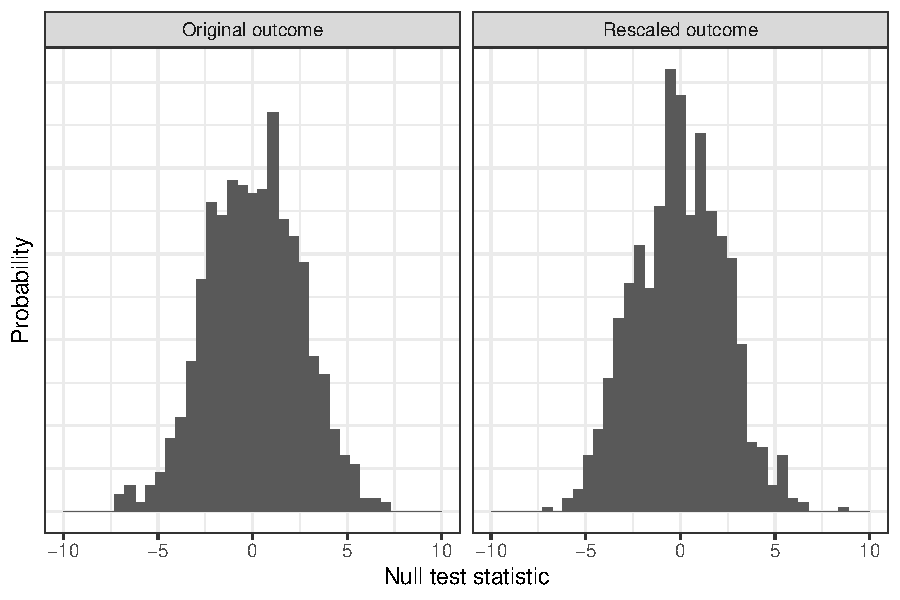
\includegraphics[width=0.9\linewidth]{null_dist_no_effect_plot.pdf}
\caption{Distribution of the Difference-in-Means test statistic under the sharp null of no effect}
\end{figure}
\end{frame}
%------------------------------------------------------------------------
\begin{frame}{Hypothesis tests in adjusted outcomes}
\vfill
\begin{itemize} 
\item How do we test hypotheses other than no effect for all units? \pause \vfill
\item Write units' true adjsuted outcomes as $\tilde{y}_i = y_i - \tau_i z_i$ for $i = 1, \ldots , N$ \vfill
\item $\bm{\tilde{y}}$ is fixed over all assignments \\ so true distribution of test-stat with adjusted outcomes, $t\left(\bm{Z}, \bm{\tilde{y}}\right)$\pause \vfill
\item So to conduct a test about $\bm{\tau}$, we can compare $t(\bm{z}, \bm{\tilde{y}}_{h})$ to the randomization distribution of $t(\bm{Z}, \bm{\tilde{y}}_{h})$, where $\tilde{y}_{hi} = y_i - z_i \tau_{hi}$ \vfill
\end{itemize}
\vfill
\end{frame}
%------------------------------------------------------------------------
\begin{frame}{Hypothesis tests in adjusted outcomes}
\begin{itemize}
\item $H_0$: GOTV campaign increases voter turnout by $p$ percentage points per precinct  
\end{itemize}
\begin{center}
  \begin{tabular}{r|rr|rrrr}
  \hline
 & GOTV? & vote03(\%)& $\bm{\tilde{y}}_h$ & $\bm{y_C}$ & $\bm{y_T}$ & $\bm{\tau}$\\
  \hline
1 & 0 & 38 & 38 & 38 & ? & ?\\
$\vdots$& & & & & & \\
13 & 0 & 19 & 19 & 19& ? & ?\\
14 & 0 & 34 & 34 & 34& ? & ?\\
15 & 1 & 49 & 49 - p & ?& 49 & ?\\
16 & 1 & 38 & 38 - p & ?& 38 & ?\\
$\vdots$& & & & & & \\
28 & 1 & 29 & 29 - p & ?& 29 & ? \\
   \hline
\end{tabular}
\end{center}
\end{frame}
%------------------------------------------------------------------------
\begin{frame}{Hypothesis tests in adjusted outcomes}
\begin{itemize}
\item For example, $H_0$: $p = 2.5$  
\end{itemize}
\begin{center}
  \begin{tabular}{r|rr|rrrr}
  \hline
 & GOTV? & vote03(\%)& $\bm{\tilde{y}}_h$ & $\bm{y_C}$ & $\bm{y_T}$ & $\bm{\tau}$\\
  \hline
1 & 0 & 38 & 38 & 38 & ? & ?\\
$\vdots$& & & & & & \\
13 & 0 & 19 & 19 & 19& ? & ?\\
14 & 0 & 34 & 34 & 34& ? & ?\\
15 & 1 & 49 & 46.5 & ?& 49 & ?\\
16 & 1 & 38 & 35.5 & ?& 38 & ?\\
$\vdots$& & & & & & \\
28 & 1 & 29 & 26.5 & ?& 29 & ? \\
   \hline
\end{tabular}
\end{center}
\begin{itemize}
\item The observed test statistic calculated on adjusted outcomes is $t(\bm{z}, \bm{\tilde{y}}_h) \approx 1.13$
\item How does it compare to $t\left(\bm{Z}, \bm{\tilde{y}}_h\right)$?
\end{itemize}
\end{frame}
%------------------------------------------------------------------------
\begin{frame}{Hypothesis tests in adjusted outcomes}
\begin{figure}[H]
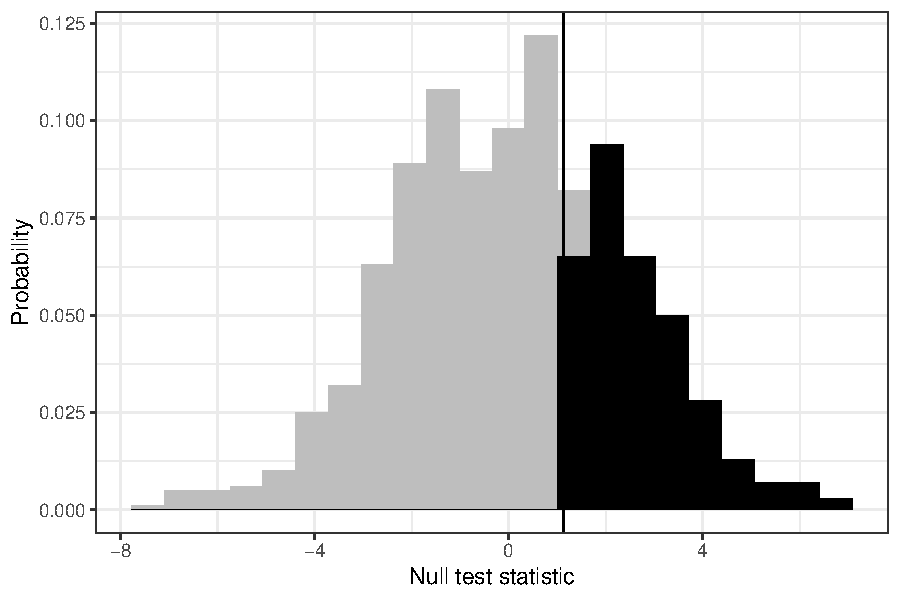
\includegraphics[width=0.9\linewidth]{null_unif_plot.pdf}
\end{figure}
\end{frame}
%------------------------------------------------------------------------
\begin{frame}{Confidence sets}
\vfill
\begin{itemize} \vfill
\item To get a confidence set we do what we just did with $p = 2.5$ over an entire grid of values of $p$ \vfill
\item A $1-\alpha$ confidence set for $p$ $= $ \{$p$: $H_{p}$ not rejected at level $\alpha$\} \vfill
\item We test over all values of $p$ and retain those we fail to reject with adjusted outcomes \vfill
\item Two sided confidence set for ACORN example: $\left\{-0.4, 7.5\right\}$ \vfill
\item We fail to reject sharp null of no effect \vfill
\end{itemize}
\end{frame}
%------------------------------------------------------------------------
\end{document}